\originalchapter{8.512作业9--12：配对与磁响应}
\psource{Patrick A. Lee，8.512 Spring 2009，公开作业9--12。}
\originalsection{作业9（2009年4月22日截止）}
\begin{exercise}[原题1(a)--(b)]\label{p:512-9-1}
取声子吸引$V_p=-V_0$在$|\omega|<\omega_D$，库仑排斥$N_\uparrow(0)V_c=\mu>0$在$|\omega|<E_F$，原题把频率作能量并取$\hbar=1$。(a)写有限温隙方程，近$T_c$试分段$\Delta_1$（低于$\omega_D$）与$\Delta_2$（高于$\omega_D$）；说明库仑项$A(\xi)$缓变且高能声子项小，导出$\mu^*=\mu/[1+\mu\log(E_F/\omega_D)]$及$1=[N_\uparrow V_0-\mu^*]\log(\omega_D/\kb T_c)$，估计典型金属参数。(b)仅考虑离子质量使$\omega_D$变化，求无库仑与有库仑的同位素系数。
\end{exercise}
\begin{solution}
完整方程$\Delta(\xi)=-N_\uparrow\int V(\xi-\xi')\Delta(\xi')\tanh(E_{\xi'}/2\kb T)/(2E_{\xi'})\dd\xi'$。近$T_c$取$E=|\xi'|$，两侧能量积分合并。宽库仑窗口$E_F$使在小$\xi$范围卷积变化缓慢，可以常数$A(0)$代替；高$\xi$的声子窗口只覆盖窄能段，其贡献无低能对数，故$\Delta_2\simeq A(0)$。令$\lambda=N_\uparrow V_0$、$L_1=\log(\omega_D/\kb T_c)$、$L_2=\log(E_F/\omega_D)$，分段方程为
\begin{equation}
\Delta_1=(\lambda-\mu)L_1\Delta_1-\mu L_2\Delta_2,\qquad\Delta_2=-\mu L_1\Delta_1-\mu L_2\Delta_2.
\end{equation}
第二式给$\Delta_2=-\mu L_1\Delta_1/(1+\mu L_2)$，回代得$1=(\lambda-\mu^*)L_1$。高能对数使有效排斥较小，例如假设$\mu=0.3,E_F/\omega_D=100$，$\mu^*=0.126$；这只是典型参数量级，不替代材料屏蔽势的计算。

(b)声子频率$\omega_D\propto M^{-1/2}$，所以$\delta\log\omega_D=-\delta\log M/2$。无排斥$T_c\propto\omega_D$，同位素指数$\alpha=-\partial\log T_c/\partial\log M=1/2$。有排斥$\partial\mu^*/\partial\log\omega_D=(\mu^*)^2$，$\log T_c=\log\omega_D-1/(\lambda-\mu^*)+\mathrm{const}$，因此$\alpha=\frac12[1-(\mu^*/(\lambda-\mu^*))^2]$。该结果固定$\lambda,E_F,\mu$，不包括结构或电子态随同位素变化。
\end{solution}
\begin{exercise}[原题2]\label{p:512-9-2}
两个类氢原子位于$R_a,R_b$，轨道$\phi_a,\phi_b$，重叠$l=\int\phi_a^*\phi_b\dd r$。定义$\Delta H=e_*^2/R_{ab}+e_*^2/r_{12}-e_*^2/r_{1b}-e_*^2/r_{2a}$，$V=\iint|\phi_a(1)\phi_b(2)|^2\Delta H$，$I=\iint\phi_a^*(1)\phi_b^*(2)\phi_b(1)\phi_a(2)\Delta H$。证明Heitler--London单重、三重能为$E_a+E_b+(V\pm I)/(1\pm|l|^2)$；若轨道实可写$l^2$。
\end{exercise}
\begin{solution}
空间态$\Psi_\pm=[\phi_a(1)\phi_b(2)\pm\phi_b(1)\phi_a(2)]/\sqrt{2(1\pm|l|^2)}$，分别配自旋反对称单重与对称三重，使总态反对称。原子哈密顿量作用给$E_a+E_b$；$\Delta H$的两对角矩阵元相等为$V$，两交叉矩阵元为$I$和$I^*$，实无流情况取$I$实。归一化相除得答案。括号只包$(V\pm I)$，不能把$E_a+E_b$也误除以重叠因子。
\end{solution}
\originalsection{作业10（2009年4月29日截止）}
\begin{exercise}[原题1(a)--(b)]\label{p:512-10-1}
(a)由线性响应证明纵向静态磁化率可用$S_{zz}(q,\omega)$的频谱积分表示，权重为$(1-\e^{-\beta\hbar\omega})/(\hbar\omega)$，取$q\to0$并明确磁矩单位。(b)若总磁化$M_z$与$H$对易，由$F=-\kb T\log\Tr\e^{-\beta(H-H_zM_z)}$导出$\chi=\beta\avg{M_z^2}$（零均值），证明与(a)一致。
\end{exercise}
\begin{solution}
(a)静态响应也可写虚时间积分$\chi=\int_0^\beta\avg{\delta M_z(-\ii\hbar\tau)\delta M_z(0)}\dd\tau$。插入能量态，$\int_0^\beta\e^{-\tau(E_m-E_n)}\dd\tau=(1-\e^{-\beta(E_m-E_n)})/(E_m-E_n)$，所以
\begin{equation}
\chi(q,0)=\int\frac{\dd\omega}{2\pi}\frac{1-\e^{-\beta\hbar\omega}}{\hbar\omega}\,S_{MM}(q,\omega).
\end{equation}
$S$若以自旋而非磁矩定义须乘$(g\mu_B)^2$，体积归一同样不能省；原题取$\hbar=1$即其表达。

(b)$[M_z,H]=0$时$\partial_{H_z}\log Z=\beta\avg{M_z}$，再求导$\chi=\beta(\avg{M_z^2}-\avg{M_z}^2)$。零場均值为0时得题示形式。谱只有$S_{MM}(0,\omega)=2\pi\avg{(\delta M_z)^2}\delta(\omega)$，权重在$\omega=0$的连续极限为$\beta$，两式一致。严格孤立守恒总量的有限频率响应与热库中等温静态导数可有极限顺序差，题目使用的是热平衡静态磁化率。
\end{solution}
\originalsection{作业11（2009年5月6日截止）}
\begin{exercise}[原题1(a)--(b)]\label{p:512-11-1}
用前题结果求三维Heisenberg反铁磁的低温沿Néel轴磁化率，证明$\chi_\parallel\propto T^2$。若有Ising易轴各向异性，说明指数激活形式并给激活隙$\Delta$。
\end{exercise}
\begin{solution}
两种反铁磁磁振子携带相反的$\Delta S_z=\pm1$，小纵场能量移$E_k\mp g\mu_BH$。每体积响应为
\begin{equation}
\chi_\parallel=2(g\mu_B)^2\int\frac{\dd^3k}{(2\pi)^3}\,\beta n_B(E_k)[1+n_B(E_k)].
\end{equation}
无各向异性$E_k=\hbar ck$，换变量$x=\beta\hbar ck$，积分$\int x^2\e^x/(\e^x-1)^2\dd x=\pi^2/3$，得$\chi_\parallel=(g\mu_B)^2(\kb T)^2/(3\hbar^3c^3)$，SI还按定义乘$\mu_0$。基态不能沿Néel轴连续极化，所以此纵向热响应趋0，横向响应则另有常数项。

有各向异性$E_k\simeq\sqrt{\Delta^2+\hbar^2c^2k^2}$，最低隙$\Delta=\sqrt{(\omega_0+\omega_A)^2-\omega_0^2}=\sqrt{\omega_A(2\omega_0+\omega_A)}$，其中题面$\omega$按能量计。低温积分进一步给$T^{1/2}\e^{-\Delta/\kb T}$前因子，因此原题的$\sim\e^{-\Delta/T}$应理解为主指数，而非无幂因子的严格等价。
\end{solution}
\begin{exercise}[原题2(a)--(b)]\label{p:512-11-2}
立方双子格反铁磁有易轴$-D(S^z)^2$，$D>0$，自旋波$E_k=\sqrt{(\omega_0+\omega_A)^2-\omega_0^2\gamma_k^2}$，$\omega_0=2zJS,\omega_A=2DS,\gamma_k=z^{-1}\sum_\delta\e^{\ii k\delta}$。(a)纵場证明两支$E_k\pm g\mu_BH_z$。(b)横場$H_y$如何改变谱？需先确定新的经典基态。
\end{exercise}
\begin{solution}
(a)磁振子的总$S_z$量子数为$\pm1$，Zeeman直接移能。纵場若超过稳定范围会发生自旋翻转，不能仍用旧Néel态。

(b)采用与题示$\omega_0$相容的$H=2J\sum_{\avg{ij}}\vct S_i\cdot\vct S_j-D\sum_i(S_i^z)^2-h\sum_iS_i^y$，$h=g\mu_BH_y$。两子格取$\vct S_A=S(0,s,c)$、$\vct S_B=S(0,s,-c)$，$s=\sin\theta,c=\cos\theta$。每站经典能$E/S^2=-zJ+(2zJ+D)s^2-hs/S-D$，极小$s=h/[2S(2zJ+D)]=h/(2\omega_0+\omega_A)$，要求$|s|<1$。

分别转到各子格局域轴后作HP展开，二次正常对角$A=\omega_0+\omega_A-(\omega_A/2)s^2$，正常子格杂化$B_k=\omega_0\gamma_ks^2$，反常子格配对$C_k=\omega_0\gamma_kc^2$，同站反常项$D_0=(\omega_A/2)s^2$。对子格对称与反对称模作玻色Bogoliubov变换，得到
\begin{equation}
E_{k,\pm}=\sqrt{(A\pm B_k)^2-(D_0\pm C_k)^2}.
\end{equation}
$h=0$恢复题示二重谱；横场修正从$h^2$开始且两支分开，并非简单的$E_k\pm h$。当$|s|\to1$达到饱和边界，旧低场分支需重新判稳定。随卷数值脚本核对$h=0$退化、正常/反常矩阵本征值与上式一致。
\end{solution}
\originalsection{作业12（2009年5月13日截止）}
\begin{exercise}[原题1--4(a)--(b)]\label{p:512-12-1}
接触排斥$U$的费米气在Stoner平均场有$\Delta=U(n_\uparrow-n_\downarrow)$，$\widetilde\epsilon_{k\uparrow}=\epsilon_k-\Delta/2$、$\widetilde\epsilon_{k\downarrow}=\epsilon_k+\Delta/2$，采用原题$\hbar=1$。(1)求自旋翻转横向响应泡图$\chi_\perp^0=\mu_B^2\Gamma_0$。(2)自洽响应证明$\chi_\perp=\mu_B^2\Gamma_0/(1-U\Gamma_0)$。(3)画单粒子--空穴连续谱在$(q,\omega)$中的支撑。(4a)证明$q=\omega=0$分母为0。(4b)小$q,\omega$展开求$\omega=Cq^2$及$C$的积分形式。
\end{exercise}
\begin{solution}
用正静态约定取
\begin{equation}
\Gamma_0(q,\omega)=\int\frac{\dd^dk}{(2\pi)^d}\frac{f(\epsilon_k-\Delta/2)-f(\epsilon_{k+q}+\Delta/2)}{\Delta+\epsilon_{k+q}-\epsilon_k-\omega-\ii0}.
\end{equation}
与原题把分子、分母同时反号的式相同，明确$k$不是两个不同的下标误排。外部横场加诱导交换场$U\delta S$，$\delta S=\Gamma_0(H+U\delta S)$，解出几何级数分母。

(3)把源题的连续色散专门取为三维各向同性抛物线$\epsilon_k=k^2/(2m)$，$T=0$，记多数与少数费米半径$a=k_{F\uparrow}>b=k_{F\downarrow}>0$，同一化学势要求$\Delta=(a^2-b^2)/(2m)$。正频率吸收只能由占据的$\uparrow$态到空的$\downarrow$态：$|k|\le a,\ |k+q|\ge b$，且
\begin{equation}
\omega=\Delta+\frac{q^2+2\vct k\cdot\vct q}{2m},\qquad q=|\vct q|.
\end{equation}
上边界取$\vct k$与$\vct q$同向、$|k|=a$，末态必在少数费米球外，故$\omega_+(q)=\Delta+q^2/(2m)+aq/m$。反向$\vct k=-a\hat q$的候选下边界$L(q)=\Delta+q^2/(2m)-aq/m$，仅在$|q-a|\ge b$时满足末态Pauli条件。若$a-b<q<a+b$，两个费米球的边界相交，可令初末态都在各自费米面上，连续谱下边界改为0。因此完整支撑是
\begin{equation}
\operatorname{Im}\chi^0_\perp(q,\omega)\ne0\quad\Longleftrightarrow\quad
\omega_-(q)<\omega<\omega_+(q),\qquad
\omega_-(q)=\begin{cases}
L(q),&0\le q\le a-b\ \text{或}\ q\ge a+b,\\
0,&a-b\le q\le a+b.
\end{cases}
\end{equation}
边界上响应可随相空间端点趋零，故用开区间表示非零内部；$q=0$连续谱退化到$\omega=\Delta$，仍有来自$b<|k|<a$的非零谱权重。两球相交的$q$区间里低频粒子--空穴态存在，不能把$\Delta\pm v_{F\uparrow}q$外推成全局下界。示意图以$a=2,b=1,m=1$取单位，此时$\Delta=3/2$、两处阈值为$q=1,3$；纵轴为正频率，阴影是允许区：
\begin{center}
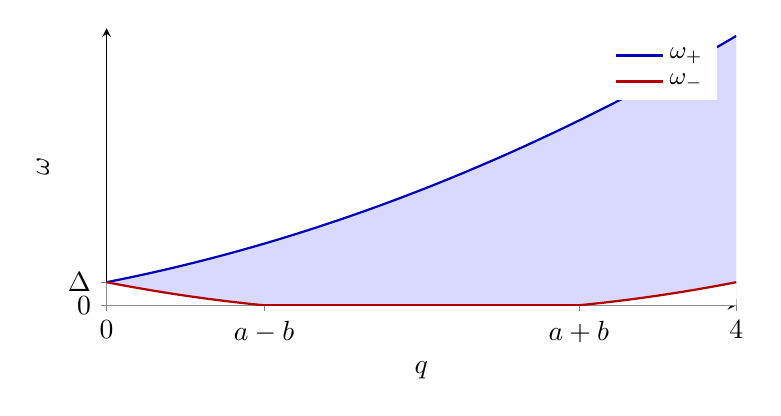
\begin{tikzpicture}
\begin{axis}[width=.79\linewidth,height=5.1cm,xmin=0,xmax=4,ymin=0,ymax=18,
 xlabel={$q$},ylabel={$\omega$},axis lines=left,xtick={0,1,3,4},
 xticklabels={$0$,$a-b$,$a+b$,$4$},ytick={0,1.5},yticklabels={$0$,$\Delta$},
 legend style={at={(.97,.97)},anchor=north east,draw=none,fill=white,font=\small}]
\addplot[forget plot,fill=blue!15,draw=none,domain=0:4,samples=100]{1.5+x*x/2+2*x}\closedcycle;
\addplot[forget plot,fill=white,draw=none,domain=0:4,samples=160]{max(0,1.5+x*x/2-2*x)}\closedcycle;
\addplot[domain=0:4,samples=100,draw=blue!70!black,thick]{1.5+x*x/2+2*x};
\addplot[domain=0:4,samples=160,draw=red!70!black,thick]{max(0,1.5+x*x/2-2*x)};
\legend{$\omega_+$,$\omega_-$}
\end{axis}
\end{tikzpicture}
\end{center}
图的$\omega_-$折到0是末态Pauli限制的几何结果，不是令自旋分裂$\Delta$消失。小$q<a-b$时Goldstone模$\omega\propto q^2$在连续谱下方；更大$q$的集体模是否衰减还要解完整响应分母。

(4a)$\Gamma_0(0,0)=(n_\uparrow-n_\downarrow)/\Delta=1/U$，正是平均场自洽式。(4b)令$A=\partial_\omega\Gamma_0|_0=(n_\uparrow-n_\downarrow)/\Delta^2$，$B=(2d)^{-1}\nabla_q^2\Gamma_0|_0$，反演对称使一阶$q$消失，则$1-U\Gamma_0\simeq-U(A\omega+Bq^2)$，所以$C=-B/A$。抛物线可先把第二项换元为$k'=k+q$，再展开两个分母，得到
\begin{equation}
B=-\frac{n}{2m\Delta^2}+\frac1{d m^2\Delta^3}\int\frac{\dd^dk}{(2\pi)^d}k^2[f(\epsilon_k-\Delta/2)-f(\epsilon_k+\Delta/2)].
\end{equation}
故$C=n/[2m(n_\uparrow-n_\downarrow)]-\int k^2(f_\uparrow-f_\downarrow)/[d m^2\Delta(n_\uparrow-n_\downarrow)]$。恢复$\hbar$时每个$k$速度与$q^2$曲率带相应$\hbar^2$。符号正表示所选均匀态的长波稳定；若算出负刚度，应审查模型态是否不稳定，不能强行叫稳定自旋波。
\end{solution}
